\documentclass[13pt,a4paper]{extarticle}

% --- Essential Packages ---
\usepackage[margin=1.5cm]{geometry}
\usepackage{amsmath,amssymb,amsfonts}
\usepackage{tikz}
\usepackage{tasks}
\usepackage{fancyhdr}
\usepackage{xcolor}
\usepackage{array}

% --- Font & Language for XeLaTeX / LuaLaTeX ---
\usepackage{fontspec}
\newfontfamily\bengalifont{Noto Serif Bengali}[
  BoldFont={Noto Serif Bengali Bold},
  Scale=1.05
]

% --- Watermark: JB PHYSICS ---
\usepackage{eso-pic}
\AddToShipoutPictureBG{%
  \begin{tikzpicture}[remember picture, overlay]
    \node[
      rotate=45,
      scale=5.0,
      text=black!8,
      font=\bfseries\sffamily
    ] at (current page.center) {JB PHYSICS};
  \end{tikzpicture}%
}

% --- Page Header & Footer ---
\pagestyle{fancy}
\fancyhf{}
\lhead{\textbf{\large Class 12 Physics — PYQ Practice}}
\rhead{\textbf{\large JB PHYSICS}}
\cfoot{\textbf{\thepage}}
\renewcommand{\headrulewidth}{0.8pt}

% Custom Command for Question Header
\newcommand{\questionheader}[1]{%
  \vspace{0.4cm}\noindent{\Large\textbf{#1}}\vspace{0.12cm}%
}

\begin{document}

% --- Header Title Banner ---
\begin{center}
  {\Huge \textbf{JB PHYSICS}}\\[4pt]
  {\LARGE \textbf{Class 12 Physics | Semester III PYQ Practice}}\\[4pt]
  \rule{\textwidth}{1.2pt}\\[4pt]
  \textbf{\large Full Marks: 35} \hfill \textbf{\large Time: 1h 15min} \hfill \textbf{\large Marks: $1 \times 35 = 35$}
\end{center}

\vspace{0.2cm}
\noindent\textit{\textbf{\large Instructions:} All questions carry 1 mark each. Choose the single correct option for each question.}
\vspace{0.3cm}

\settasks{label=(\Alph*), label-width=4ex, item-indent=1.5em, column-sep=1.2em}

% ==================== QUESTION 1 ====================
\questionheader{Question 1}

{\bengalifont কোনো অঞ্চলে ক্রিয়াশীল তড়িৎক্ষেত্র হল $\vec{E} = (3\hat{i} - 4\hat{j} + 2\hat{k})\text{ V/m}$; ওই অঞ্চলে $YZ$-তলে অবস্থিত $2\text{ m}$ বাহুবিশিষ্ট বর্গাকার ক্ষেত্রের মধ্য দিয়ে অতিক্রান্ত তড়িৎ ফ্লাক্স হল—}

\vspace{0.08cm}
\textit{The electric field in a region is $\vec{E} = (3\hat{i} - 4\hat{j} + 2\hat{k})\text{ V/m}$. The electric flux passing through a square region of side $2\text{ m}$ situated in the $YZ$-plane in that region is:}

\begin{tasks}(4)
  \task $12\text{ V}\cdot\text{m}$
  \task $6\text{ V}\cdot\text{m}$
  \task $-16\text{ V}\cdot\text{m}$
  \task $8\text{ V}\cdot\text{m}$
\end{tasks}

% ==================== QUESTION 2 ====================
\questionheader{Question 2}

{\bengalifont একটি সমান্তরাল পাতধারকের পাতদ্বয়ের মধ্যবর্তী মাধ্যমের পরাবৈদ্যুতিক ধ্রুবক $2$। এর ধারকত্ব $3\,\mu\text{F}$। এখন, ধারকটির পাতদ্বয়ের মধ্যবর্তী দূরত্ব দ্বিগুণ করে, ওই ফাঁকা স্থানে $k = 4$ পরাবৈদ্যুতিক ধ্রুবকসম্পন্ন প্লেট প্রবেশ করানো হল। এখন ধারকটির ধারকত্ব হবে—}

\vspace{0.08cm}
\textit{The dielectric constant of the medium between the plates of a parallel plate capacitor is $2$. Its capacitance is $3\,\mu\text{F}$. Now, the distance between the plates is doubled and a plate of dielectric constant $k = 4$ is inserted into that space. Now the capacitance of the capacitor will be:}

\begin{tasks}(4)
  \task $1\,\mu\text{F}$
  \task $2\,\mu\text{F}$
  \task $6\,\mu\text{F}$
  \task $9\,\mu\text{F}$
\end{tasks}

% ==================== QUESTION 3 ====================
\questionheader{Question 3}

{\bengalifont দুটি পরিবাহী $X$ এবং $Y$-এর ধারকত্ব যথাক্রমে $3C$ এবং $C$। পরিবাহী $X$-এ $Q$ আধান দেওয়া হল যা পরিবাহীটি $Y$-এর সঙ্গে ভাগ করে নেয়। ভাগ হওয়ার পরে মোট শক্তি এবং মোট প্রাথমিক শক্তির অনুপাত হবে—}

\vspace{0.08cm}
\textit{Two conductors $X$ and $Y$ have capacitances $3C$ and $C$ respectively. A charge $Q$ is given to conductor $X$, which is then shared with conductor $Y$. The ratio of total energy after sharing to total initial energy will be:}

\begin{tasks}(4)
  \task $9:16$
  \task $\sqrt{3}:2$
  \task $3:4$
  \task $4:3$
\end{tasks}

% ==================== QUESTION 4 ====================
\questionheader{Question 4}

{\bengalifont
নিম্নলিখিত বিবৃতিগুলির মধ্যে কোনটি/কোনগুলি সঠিক তা চিহ্নিত করো:\\
$l$ দৈর্ঘ্যবিশিষ্ট ও $A$ প্রস্থচ্ছেদবিশিষ্ট কোনো পরিবাহীর দু-প্রান্তে $V$ বিভবপ্রভেদ প্রয়োগ করা হল।\\
\textbf{বিবৃতি I :} বিভবপ্রভেদ দ্বিগুণ করা হলে তড়িৎপ্রবাহ ঘনত্ব দ্বিগুণ হবে।\\
\textbf{বিবৃতি II :} বিভবপ্রভেদ দ্বিগুণ করা হলে বিচলন বেগ অর্ধেক হয়ে যাবে।\\
\textbf{বিবৃতি III :} প্রস্থচ্ছেদ দ্বিগুণ করা হলে তড়িৎপ্রবাহ ঘনত্ব কমে যাবে।
}

\vspace{0.08cm}
\textit{Identify which of the following statement(s) is/are correct:\\
A potential difference $V$ is applied across the ends of a conductor of length $l$ and cross-sectional area $A$.\\
\textbf{Statement I:} If the potential difference is doubled, current density will be doubled.\\
\textbf{Statement II:} If the potential difference is doubled, drift velocity will become half.\\
\textbf{Statement III:} If the cross-sectional area is doubled, current density will decrease.}

\begin{tasks}(2)
  \task {\bengalifont I এবং II সঠিক} / I and II are correct
  \task {\bengalifont কেবলমাত্র I সঠিক} / Only I is correct
  \task {\bengalifont কেবলমাত্র III সঠিক} / Only III is correct
  \task {\bengalifont II এবং III সঠিক} / II and III are correct
\end{tasks}

% ==================== QUESTION 5 ====================
\questionheader{Question 5}

{\bengalifont ধরা যাক $l$ দৈর্ঘ্যবিশিষ্ট একটি তারের রোধ হল $R$। এখন তারটিকে ততক্ষণ টানা হল যতক্ষণ না তারটির দৈর্ঘ্য পূর্বের $x$ গুণ হয়। এখন তারটির রোধ হবে—}

\vspace{0.08cm}
\textit{Let the resistance of a wire of length $l$ be $R$. Now the wire is stretched until its length becomes $x$ times the initial length. Now the resistance of the wire will be:}

\begin{tasks}(4)
  \task $x^2 R$
  \task $x R$
  \task $\dfrac{R}{x}$
  \task $R$
\end{tasks}

% ==================== QUESTION 6 ====================
\questionheader{Question 6}

{\bengalifont অ্যাম্পিয়ারের বর্তনী সূত্র অনুযায়ী একটি আদর্শ সলিনয়েডের অক্ষে চৌম্বক ক্ষেত্রপ্রাবল্য $B$ এবং এর ব্যাসার্ধ $r$ হলে—}

\vspace{0.08cm}
\textit{According to Ampere's circuital law, for an ideal solenoid, the magnetic field strength $B$ on its axis and its radius $r$ are related as:}

\begin{tasks}(2)
  \task $B \propto r$
  \task $B \propto \dfrac{1}{r}$
  \task $B \propto \dfrac{1}{r^2}$
  \task {\bengalifont $B$, $r$-এর নিরপেক্ষ} / $B$ is independent of $r$
\end{tasks}

% ==================== QUESTION 7 ====================
\questionheader{Question 7}

{\bengalifont একটি ভোল্টমিটারের রোধ $300\,\Omega$। যন্ত্রটি $150\text{ V}$ সর্বোচ্চ বিভবপার্থক্য পরিমাপ করতে পারে। যন্ত্রটিকে $8\text{ A}$ পর্যন্ত প্রবাহমাত্রা মাপার উপযুক্ত অ্যামিটারে পরিণত করতে হলে যে রোধ যুক্ত করতে হবে, তা হল—}

\vspace{0.08cm}
\textit{The resistance of a voltmeter is $300\,\Omega$. The instrument can measure a maximum potential difference of $150\text{ V}$. To convert this instrument into an ammeter capable of measuring currents up to $8\text{ A}$, the resistance to be connected is:}

\begin{tasks}(2)
  \task $20\,\Omega$, {\bengalifont সমান্তরালে} / in parallel
  \task $20\,\Omega$, {\bengalifont শ্রেণিতে} / in series
  \task $30\,\Omega$, {\bengalifont সমান্তরালে} / in parallel
  \task $40\,\Omega$, {\bengalifont শ্রেণিতে} / in series
\end{tasks}

% ==================== QUESTION 8 ====================
\questionheader{Question 8}

{\bengalifont অর্ধবৃত্তাকার পরিবাহীর ক্ষেত্রে (চিত্রে দেখানো হয়েছে): পরিবাহীর কেন্দ্রবিন্দুতে চৌম্বক ক্ষেত্র হবে—}

\vspace{0.08cm}
\textit{For the semicircular conductor (as shown in the figure): the magnetic field at the center of the conductor will be:}

\begin{center}
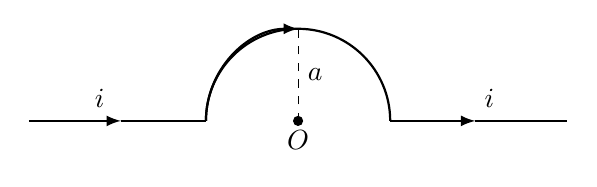
\begin{tikzpicture}[scale=0.9, >=latex]
    \draw[thick, ->] (-2.5, 0) -- (-1.2, 0);
    \draw[thick] (-1.2, 0) -- (0, 0);
    \node[above] at (-1.5, 0.05) {$i$};
    \draw[thick, ->] (0,0) arc (180:90:1.3);
    \draw[thick] (0,0) arc (180:0:1.3);
    \filldraw (1.3, 0) circle (1.8pt) node[below] {$O$};
    \draw[dashed] (1.3, 0) -- (1.3, 1.3);
    \node[right] at (1.3, 0.65) {$a$};
    \draw[thick, ->] (2.6, 0) -- (3.8, 0);
    \draw[thick] (3.8, 0) -- (5.1, 0);
    \node[above] at (4.0, 0.05) {$i$};
\end{tikzpicture}
\end{center}

\begin{tasks}(4)
  \task $\dfrac{\mu_0 i}{2a}$
  \task $\dfrac{\mu_0 i}{2\pi a}$
  \task {\bengalifont শূন্য} / Zero
  \task $\dfrac{\mu_0 i}{4a}$
\end{tasks}

% ==================== QUESTION 9 ====================
\questionheader{Question 9}

{\bengalifont কোনো একস্থানে পৃথিবীর চৌম্বক ক্ষেত্রের উল্লম্ব উপাংশ অনুভূমিক উপাংশের দ্বিগুণ। ওই স্থানে বিনতি কোণ $\theta$ হলে, $\tan\theta$-এর মান হবে—}

\vspace{0.08cm}
\textit{At a certain place, the vertical component of Earth's magnetic field is twice the horizontal component. If the angle of dip at that place is $\theta$, the value of $\tan\theta$ will be:}

\begin{tasks}(4)
  \task $2$
  \task $\dfrac{1}{2}$
  \task $\dfrac{1}{\sqrt{3}}$
  \task $\sqrt{3}$
\end{tasks}

% ==================== QUESTION 10 ====================
\questionheader{Question 10}

{\bengalifont $1\text{ m}$ বাহু এবং $1\,\Omega$ রোধবিশিষ্ট একটি বর্গাকার কুণ্ডলীকে $0.5\text{ T}$ চৌম্বক ক্ষেত্রে রাখা আছে। যদি কুণ্ডলীর তল চৌম্বক ক্ষেত্রের অভিমুখের সঙ্গে লম্ব হয়, তাহলে কুণ্ডলীর মধ্যে দিয়ে চৌম্বক প্রবাহ হবে—}

\vspace{0.08cm}
\textit{A square coil of side $1\text{ m}$ and resistance $1\,\Omega$ is placed in a magnetic field of $0.5\text{ T}$. If the plane of the coil is perpendicular to the direction of the magnetic field, then the magnetic flux through the coil will be:}

\begin{tasks}(4)
  \task $0.5\text{ weber}$
  \task $1\text{ weber}$
  \task $0\text{ weber}$
  \task $2\text{ weber}$
\end{tasks}

% ==================== QUESTION 11 ====================
\questionheader{Question 11}

{\bengalifont কোনো তিরশ্চৌম্বক পদার্থের ক্ষেত্রে কোনটি সঠিক?}

\vspace{0.08cm}
\textit{For a diamagnetic material, which of the following is correct?}

\begin{tasks}(4)
  \task $B = H$
  \task $B < H$
  \task $B > H$
  \task $B \gg H$
\end{tasks}

% ==================== QUESTION 12 ====================
\questionheader{Question 12}

{\bengalifont একটি ইস্পাতের তারের চৌম্বক ভ্রামক $M$। এটিকে বাঁকিয়ে অর্ধবৃত্তাকার করা হলে তারটির নতুন চৌম্বক ভ্রামক হবে—}

\vspace{0.08cm}
\textit{The magnetic dipole moment of a steel wire is $M$. If it is bent into a semicircle, the new magnetic dipole moment of the wire will be:}

\begin{tasks}(4)
  \task $M$
  \task $\dfrac{2M}{\pi}$
  \task $\dfrac{M}{2\pi}$
  \task $\dfrac{M}{\pi}$
\end{tasks}

% ==================== QUESTION 13 ====================
\questionheader{Question 13}

{\bengalifont দুটি সমান্তরাল তড়িৎবাহী তারের মধ্যে ক্রিয়াশীল বল $F$। যদি প্রতিটি তারের প্রবাহ দ্বিগুণ ও মধ্যবর্তী দূরত্ব তিনগুণ করা হয়, তাহলে তাদের মধ্যে ক্রিয়াশীল বল হবে—}

\vspace{0.08cm}
\textit{The force acting between two parallel current-carrying wires is $F$. If the current in each wire is doubled and the distance between them is tripled, the force acting between them will be:}

\begin{tasks}(4)
  \task $12 F$
  \task $\dfrac{4F}{3}$
  \task $\dfrac{4F}{9}$
  \task $\dfrac{2F}{9}$
\end{tasks}

% ==================== QUESTION 14 ====================
\questionheader{Question 14}

{\bengalifont দুটি বৃত্তাকার কুণ্ডলীর ব্যাসার্ধের অনুপাত $1:2$। এদের চৌম্বক ভ্রামকের অনুপাত $1:2$ হলে, এদের মধ্যে দিয়ে প্রবাহিত তড়িৎপ্রবাহের অনুপাত হবে—}

\vspace{0.08cm}
\textit{The ratio of the radii of two circular coils is $1:2$. If the ratio of their magnetic moments is $1:2$, the ratio of the electric currents flowing through them will be:}

\begin{tasks}(4)
  \task $1:1$
  \task $2:1$
  \task $4:1$
  \task $1:4$
\end{tasks}

% ==================== QUESTION 15 ====================
\questionheader{Question 15}

{\bengalifont কোন্ ক্ষেত্রে হুইটস্টোন ব্রিজের নিষ্পন্দ অবস্থাটি পরিবর্তিত হবে?}

\vspace{0.08cm}
\textit{In which case will the null condition (balanced state) of a Wheatstone bridge change?}

\begin{tasks}(1)
  \task {\bengalifont বিভিন্ন বাহুর রোধগুলিকে পরিবর্তিত করা হলে} / If the resistances of the different arms are changed
  \task {\bengalifont ব্যাটারির ও গ্যালাভানোমিটারের অবস্থান বিনিময় করা হলে} / If positions of battery and galvanometer are interchanged
  \task {\bengalifont অন্য তড়িৎচালক বলের ব্যাটারি নিলে} / If a battery of different EMF is used
  \task {\bengalifont অন্য রোধের গ্যালাভানোমিটার নিলে} / If a galvanometer of different resistance is used
\end{tasks}

% ==================== QUESTION 16 ====================
\questionheader{Question 16}

{\bengalifont নীচের চিত্রে একটি তড়িৎক্ষেত্রের বলরেখা দেখানো হয়েছে। কোন্ বিন্দুতে তড়িৎ ক্ষেত্রপ্রাবলের মান সবথেকে বেশি?}

\vspace{0.08cm}
\textit{The electric field lines in a region are shown in the figure below. At which point is the electric field intensity the greatest?}

\begin{center}
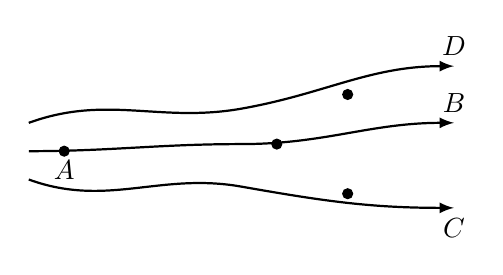
\begin{tikzpicture}[scale=0.9, >=latex]
    \draw[thick, ->] (-3, 0.4) to[out=20, in=190] (0, 0.6) to[out=10, in=180] (3, 1.2) node[above] {$D$};
    \draw[thick, ->] (-3, 0.0) to[out=0, in=180] (0, 0.1) to[out=0, in=180] (3, 0.4) node[above] {$B$};
    \draw[thick, ->] (-3, -0.4) to[out=-20, in=170] (0, -0.5) to[out=-10, in=180] (3, -0.8) node[below] {$C$};
    \filldraw (-2.5, 0.0) circle (2pt) node[below] {$A$};
    \filldraw (0.5, 0.1) circle (2pt);
    \filldraw (1.5, 0.8) circle (2pt);
    \filldraw (1.5, -0.6) circle (2pt);
\end{tikzpicture}
\end{center}

\begin{tasks}(4)
  \task $A$
  \task $B$
  \task $C$
  \task $D$
\end{tasks}

% ==================== QUESTION 17 ====================
\questionheader{Question 17}

{\bengalifont বায়ু মাধ্যমে থাকা দুটি বিন্দু-আধান পরস্পরের থেকে $0.18\text{ m}$ দূরে আছে। একটি আধানের মান অপরটির $4$ গুণ। আধান দুটির সংযোগকারী রেখার ওপর একটি বিন্দুতে তড়িৎক্ষেত্রের মান শূন্য হলে, বিন্দুটির অবস্থান হবে—}

\vspace{0.08cm}
\textit{Two point charges in air are separated by a distance of $0.18\text{ m}$. One charge is $4$ times the other. If the electric field is zero at a point on the line joining the two charges, the position of that point is:}

\begin{tasks}(1)
  \task {\bengalifont রেখার ওপর আধান দুটির বাইরে এবং বৃহত্তর আধান থেকে $0.06\text{ m}$ দূরে} / outside the two charges on the line and $0.06\text{ m}$ from the larger charge
  \task {\bengalifont রেখার ওপর আধান দুটির মধ্যবর্তী স্থানে এবং ক্ষুদ্রতর আধান থেকে $0.06\text{ m}$ দূরে} / between the two charges on the line and $0.06\text{ m}$ from the smaller charge
  \task {\bengalifont রেখার ওপর আধান দুটির মধ্যবর্তী স্থানে এবং বৃহত্তর আধান থেকে $0.04\text{ m}$ দূরে} / between the two charges on the line and $0.04\text{ m}$ from the larger charge
  \task {\bengalifont রেখার ওপর আধান দুটির বাইরে এবং ক্ষুদ্রতর আধান থেকে $0.04\text{ m}$ দূরে} / outside the two charges on the line and $0.04\text{ m}$ from the smaller charge
\end{tasks}

% ==================== QUESTION 18 ====================
\questionheader{Question 18}

{\bengalifont একটি তড়িৎ দ্বিমেরুর কেন্দ্র থেকে $r$ দূরত্বে অক্ষীয় অবস্থানে কোনো বিন্দুতে তড়িৎ ক্ষেত্রপ্রাবল্য $E$। দ্বিমেরুটিকে উল্লম্ব অক্ষের সাপেক্ষে $90^\circ$ কোণে ঘোরানো হল। এখন ওই আগের বিন্দুতে তড়িৎ ক্ষেত্রপ্রাবল্য হবে—}

\vspace{0.08cm}
\textit{The electric field intensity at an axial point at a distance $r$ from the center of an electric dipole is $E$. The dipole is rotated by $90^\circ$ about a perpendicular axis. Now the electric field intensity at that same point will be:}

\begin{tasks}(4)
  \task $E$
  \task $\dfrac{E}{4}$
  \task $\dfrac{E}{2}$
  \task $2E$
\end{tasks}

% ==================== QUESTION 19 ====================
\questionheader{Question 19}

{\bengalifont ধরা যাক, ধনাত্মক আধানে আহিত একটি অসীম পাতলা সমতল পাতের তলমাত্রিক আধান ঘনত্ব হল $\sigma$। পাতটির কাছাকাছি $r$ দূরত্বে P বিন্দুতে তড়িৎক্ষেত্রের প্রাবলের মান হল $E$। দূরত্বের সঙ্গে তড়িৎক্ষেত্রের মান কীভাবে পরিবর্তিত হবে?}

\vspace{0.08cm}
\textit{Let the surface charge density of an infinite thin plane sheet of positive charge be $\sigma$. The electric field intensity at a nearby point P at distance $r$ is $E$. How does the electric field vary with distance $r$?}

\begin{tasks}(2)
  \task $E \propto 1/r^2$ বক্ররেখা / Hyperbolic
  \task রৈখিক পরিবর্তন / Linear piecewise
  \task মূলবিন্দুগামী সরলরেখা / Proportional line
  \task অনুভূমিক সরলরেখা (দূরত্ব নিরপেক্ষ) / Constant line
\end{tasks}

% ==================== QUESTION 20 ====================
\questionheader{Question 20}

{\bengalifont $1.0\,\mu\text{F}$, $2.0\,\mu\text{F}$ এবং $5.0\,\mu\text{F}$ ধারকত্বের তিনটি ধারক একটি $10\text{ V}$ উৎসের সঙ্গে শ্রেণি সমবায়ে যুক্ত। $2.0\,\mu\text{F}$ ধারকত্বের ধারকটির দুই প্রান্তের বিভবপার্থক্য হবে—}

\vspace{0.08cm}
\textit{Three capacitors of capacitances $1.0\,\mu\text{F}$, $2.0\,\mu\text{F}$ and $5.0\,\mu\text{F}$ are connected in series with a $10\text{ V}$ source. The potential difference across the $2.0\,\mu\text{F}$ capacitor will be:}

\begin{tasks}(4)
  \task $\dfrac{100}{17}\text{ V}$
  \task $\dfrac{20}{17}\text{ V}$
  \task $\dfrac{50}{17}\text{ V}$
  \task $10\text{ V}$
\end{tasks}

% ==================== QUESTION 21 ====================
\questionheader{Question 21}

{\bengalifont পারস্পরিক আবেশ গুণাঙ্কের মাত্রীয় সংকেত হল—}

\vspace{0.08cm}
\textit{The dimensional formula of mutual inductance is:}

\begin{tasks}(4)
  \task $\text{ML}^2\text{T}^{-2}\text{I}^2$
  \task $\text{ML}^2\text{T}^{-2}\text{I}^{-2}$
  \task $\text{ML}^{-2}\text{T}^2\text{I}^2$
  \task $\text{ML}^{-2}\text{T}^{-2}\text{I}^{-2}$
\end{tasks}

% ==================== QUESTION 22 ====================
\questionheader{Question 22}

{\bengalifont
\textbf{বিবৃতি I :} পরিবর্তী প্রবাহের (ac) তুলনায় সমপ্রবাহ (dc) কম বিপজ্জনক।\\
\textbf{বিবৃতি II :} পরিবর্তী প্রবাহমাত্রার (ac) rms মান শীর্ষমানের 70.7\%।
}

\vspace{0.08cm}
\textit{\textbf{Statement I:} Direct current (dc) is less dangerous than alternating current (ac).\\
\textbf{Statement II:} The rms value of alternating current (ac) is 70.7\% of its peak value.}

\begin{tasks}(2)
  \task {\bengalifont শুধুমাত্র বিবৃতি I সত্য} / Only Statement I is true
  \task {\bengalifont শুধুমাত্র বিবৃতি II সত্য} / Only Statement II is true
  \task {\bengalifont বিবৃতি I ও II উভয়ই সত্য} / Both Statements I and II are true
  \task {\bengalifont বিবৃতি I ও II উভয়ই মিথ্যা} / Both Statements I and II are false
\end{tasks}

% ==================== QUESTION 23 ====================
\questionheader{Question 23}

{\bengalifont শূন্য মাধ্যমে একটি তড়িৎচুম্বকীয় তরঙ্গ $X$-অক্ষ বরাবর গতিশীল। যদি কোনো একটি নির্দিষ্ট অবস্থানে এবং সময়ে $\vec{B}$-এর মান $2.4 \times 10^{-8} \hat{k}\text{ tesla}$ হয়, তাহলে ওই বিন্দুতে $\vec{E}$, V/m এককে হবে—}

\vspace{0.08cm}
\textit{An electromagnetic wave is propagating along the $+X$-axis in vacuum. If at a particular location and time, the magnetic field is $\vec{B} = 2.4 \times 10^{-8}\hat{k}\text{ tesla}$, then at that point $\vec{E}$ in V/m will be:}

\begin{tasks}(4)
  \task $7.2\,\hat{j}$
  \task $7.2\,\hat{i}$
  \task $0.8\,\hat{k}$
  \task $2.4\,\hat{k}$
\end{tasks}

% ==================== QUESTION 24 ====================
\questionheader{Question 24}

{\bengalifont স্তম্ভ-I এর সাথে স্তম্ভ-II মেলাও এবং সঠিক উত্তরটি বেছে নাও:\\
স্তম্ভ-১ (তড়িৎচুম্বকীয় তরঙ্গ): (i) অবলোহিত তরঙ্গ, (ii) মাইক্রো তরঙ্গ, (iii) X-রশ্মি, (iv) রেডিও তরঙ্গ\\
স্তম্ভ-২ (তরঙ্গদৈর্ঘ্য): (a) $10^{-2}\text{ m}$, (b) $10^3\text{ m}$, (c) $10^{-7}\text{ m}$, (d) $10^{-9}\text{ m}$}

\vspace{0.08cm}
\textit{Match Column-I with Column-II and choose the correct answer:\\
Column-I: (i) Infrared waves, (ii) Microwaves, (iii) X-rays, (iv) Radio waves\\
Column-II: (a) $10^{-2}\text{ m}$, (b) $10^3\text{ m}$, (c) $10^{-7}\text{ m}$, (d) $10^{-9}\text{ m}$}

\begin{tasks}(2)
  \task (i)-(d), (ii)-(a), (iii)-(b), (iv)-(c)
  \task (i)-(d), (ii)-(c), (iii)-(b), (iv)-(a)
  \task (i)-(c), (ii)-(d), (iii)-(a), (iv)-(b)
  \task (i)-(c), (ii)-(a), (iii)-(d), (iv)-(b)
\end{tasks}

% ==================== QUESTION 25 ====================
\questionheader{Question 25}

{\bengalifont তড়িৎভেদ্যতা $\dfrac{\varepsilon_0}{2}$ এবং চৌম্বক ভেদ্যতা $2\mu_0$ বিশিষ্ট একটি মাধ্যমে তড়িৎচুম্বকীয় বিকিরণ-এর বেগ হল—}

\vspace{0.08cm}
\textit{The velocity of electromagnetic radiation in a medium having permittivity $\dfrac{\varepsilon_0}{2}$ and permeability $2\mu_0$ is:}

\begin{tasks}(4)
  \task $2\sqrt{\dfrac{\varepsilon_0}{\mu_0}}$
  \task $2\sqrt{\mu_0\varepsilon_0}$
  \task $\dfrac{1}{\sqrt{\mu_0\varepsilon_0}}$
  \task $\dfrac{1}{2}\sqrt{\dfrac{\mu_0}{\varepsilon_0}}$
\end{tasks}

% ==================== QUESTION 26 ====================
\questionheader{Question 26}

{\bengalifont নীচে দেওয়া বর্তনীতে A এবং B বিন্দু দুটির মধ্যে তুল্য রোধ হবে—}

\vspace{0.08cm}
\textit{The equivalent resistance between points A and B in the circuit network shown below will be:}

\begin{tasks}(4)
  \task $4\,\Omega$
  \task $1\,\Omega$
  \task $3\,\Omega$
  \task $2\,\Omega$
\end{tasks}

% ==================== QUESTION 27 ====================
\questionheader{Question 27}

{\bengalifont একটি পোটেনশিওমিটার তারের দৈর্ঘ্য $100\text{ cm}$ এবং রোধ $10\,\Omega$। এটি $R$ এবং $2\text{ V}$ তড়িৎচালক বল এবং নগণ্য অভ্যন্তরীণ রোধবিশিষ্ট একটি সঞ্চায়ক কোষের সঙ্গে শ্রেণিতে যুক্ত আছে। $10\text{ mV}$ তড়িৎচালক বলের একটি উৎস পোটেনশিওমিটার তারের $40\text{ cm}$ দৈর্ঘ্যের সঙ্গে প্রতিমিত হয়। ওহম এককে $R$-এর মান কত?}

\vspace{0.08cm}
\textit{A potentiometer wire has length $100\text{ cm}$ and resistance $10\,\Omega$. It is connected in series with a resistance $R$ and a $2\text{ V}$ accumulator of negligible internal resistance. A source of EMF $10\text{ mV}$ is balanced against a length of $40\text{ cm}$ of the potentiometer wire. What is the value of $R$ in ohms?}

\begin{tasks}(4)
  \task $700$
  \task $750$
  \task $790$
  \task $800$
\end{tasks}

% ==================== QUESTION 28 ====================
\questionheader{Question 28}

{\bengalifont 18টি সদৃশ তড়িৎকোষকে মিশ্র সমবায়ে এরূপভাবে সাজানো হল যাতে একটি বহিঃস্থ রোধের মধ্য দিয়ে সর্বোচ্চ প্রবাহ যায়। যদি 6টি কোষ শ্রেণি সমবায়ে এবং এরূপ সমান্তরাল সারি যুক্ত থাকে, তাহলে বহিঃস্থ রোধ এবং একটি কোষের অভ্যন্তরীণ রোধের অনুপাত হল—}

\vspace{0.08cm}
\textit{18 identical cells are grouped in a mixed combination to deliver maximum current through an external resistor. If 6 cells are in series in each row and there are 3 parallel rows, the ratio of the external resistance to the internal resistance of one cell ($R : r$) is:}

\begin{tasks}(4)
  \task $10:1$
  \task $5:1$
  \task $4:1$
  \task $2:1$
\end{tasks}

% ==================== QUESTION 29 ====================
\questionheader{Question 29}

{\bengalifont চিত্রে তিনটি ভিন্ন উষ্ণতায় ($T_1$, $T_2$ এবং $T_3$) একটি ধাতব তারের I-V লেখচিত্র দেখানো হয়েছে। এক্ষেত্রে এই সিদ্ধান্তে আসা যায় যে—}

\vspace{0.08cm}
\textit{The $I\text{-}V$ characteristics of a metallic wire at three different temperatures ($T_1$, $T_2$, and $T_3$) are shown in the figure. In this case, it can be concluded that:}

\begin{center}
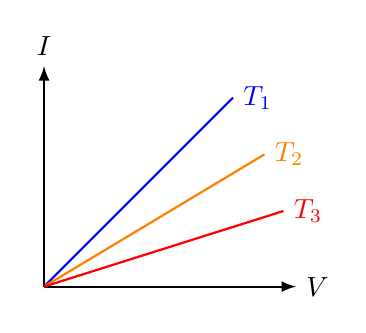
\begin{tikzpicture}[scale=0.8, >=latex]
    \draw[->, thick] (0,0) -- (4,0) node[right] {$V$};
    \draw[->, thick] (0,0) -- (0,3.5) node[above] {$I$};
    \draw[thick, blue] (0,0) -- (3,3) node[right] {$T_1$};
    \draw[thick, orange] (0,0) -- (3.5,2.1) node[right] {$T_2$};
    \draw[thick, red] (0,0) -- (3.8,1.2) node[right] {$T_3$};
\end{tikzpicture}
\end{center}

\begin{tasks}(2)
  \task $T_1 > T_2 > T_3$
  \task $T_1 < T_2 < T_3$
  \task $T_1 = T_2 = T_3$
  \task $T_1 = T_2 > T_3$
\end{tasks}

% ==================== QUESTION 30 ====================
\questionheader{Question 30}

{\bengalifont চিত্রে A এবং B দুটি তড়িৎকোষ সমান্তরালে যুক্ত। ওদের তড়িৎচালক বল যথাক্রমে 3 volt এবং 2 volt। অভ্যন্তরীণ রোধ যথাক্রমে $0.2\,\Omega$ এবং $0.3\,\Omega$। সমবায়টির তুল্য তড়িৎচালক বল হল—}

\vspace{0.08cm}
\textit{Two cells A and B are connected in parallel. Their EMFs are $3\text{ V}$ and $2\text{ V}$ respectively, and their internal resistances are $0.2\,\Omega$ and $0.3\,\Omega$ respectively. The equivalent EMF of the combination is:}

\begin{tasks}(4)
  \task $5\text{ volt}$
  \task $1\text{ volt}$
  \task $2.4\text{ volt}$
  \task $2.6\text{ volt}$
\end{tasks}

% ==================== QUESTION 31 ====================
\questionheader{Question 31}

{\bengalifont একটি ট্রান্সফরমারের 500 পাকের প্রাথমিক কুণ্ডলীতে প্রবাহ হল $4\text{ A}$। ইনপুট ক্ষমতা $1\text{ kW}$ হলে, গৌণ কুণ্ডলীর কত পাকসংখ্যার জন্য আউটপুট $500\text{ V}$ পাওয়া যাবে?}

\vspace{0.08cm}
\textit{In a transformer with 500 turns in the primary coil, the primary current is $4\text{ A}$. If the input power is $1\text{ kW}$, what number of turns in the secondary coil is required to obtain an output of $500\text{ V}$?}

\begin{tasks}(4)
  \task $1000$
  \task $400$
  \task $2000$
  \task $1500$
\end{tasks}

% ==================== QUESTION 32 ====================
\questionheader{Question 32}

{\bengalifont ac বর্তনীর অর্ধচক্রের জন্য তড়িৎপ্রবাহের rms মান ও গড় মানের অনুপাত হল—}

\vspace{0.08cm}
\textit{For a half-cycle of an AC circuit, the ratio of the rms value to the average value of alternating current is:}

\begin{tasks}(4)
  \task $\sqrt{2} : \pi$
  \task $\sqrt{2} : 1$
  \task $2\sqrt{2} : \pi$
  \task $\pi : 2\sqrt{2}$
\end{tasks}

% ==================== QUESTION 33 ====================
\questionheader{Question 33}

{\bengalifont একটি LCR শ্রেণি বর্তনীতে সর্বোচ্চ প্রবাহ পাওয়ার শর্ত হল—}

\vspace{0.08cm}
\textit{The condition to obtain maximum current in a series LCR circuit is:}

\begin{tasks}(4)
  \task $X_L = 0$
  \task $X_C = 0$
  \task $X_L = X_C$
  \task $R = X_L - X_C$
\end{tasks}

% ==================== QUESTION 34 ====================
\questionheader{Question 34}

{\bengalifont একটি পরিবর্তী তড়িৎচালক বলের সমীকরণ $E = 220 \sin\left(100\pi t - \dfrac{\pi}{15}\right)\text{ V}$, যেখানে $t$ সেকেন্ড এককে প্রকাশিত। এর rms মান ও কম্পাঙ্ক যথাক্রমে হয়—}

\vspace{0.08cm}
\textit{The equation of an alternating EMF is $E = 220 \sin\left(100\pi t - \dfrac{\pi}{15}\right)\text{ V}$, where $t$ is in seconds. Its rms value and frequency are respectively:}

\begin{tasks}(2)
  \task $\dfrac{220}{\sqrt{2}}\text{ V}, 50\text{ Hz}$
  \task $220\text{ V}, 50\text{ Hz}$
  \task $\dfrac{220}{\sqrt{2}}\text{ V}, 100\text{ Hz}$
  \task $220\sqrt{2}\text{ V}, 50\text{ Hz}$
\end{tasks}

% ==================== QUESTION 35 ====================
\questionheader{Question 35}

{\bengalifont $7\,\Omega$ রোধের একটি বর্তনীতে চৌম্বক প্রবাহের রাশিমালা $\phi = 6t^2 - 5t + 4$ হলে $t = 1\text{ s}$-এ আবিষ্ট তড়িৎপ্রবাহমাত্রা হবে—}

\vspace{0.08cm}
\textit{The magnetic flux in a circuit of resistance $7\,\Omega$ is given by $\phi = 6t^2 - 5t + 4\text{ Wb}$. The induced current at time $t = 1\text{ s}$ will be:}

\begin{tasks}(4)
  \task $1.2\text{ A}$
  \task $0.8\text{ A}$
  \task $0.5\text{ A}$
  \task $1\text{ A}$
\end{tasks}

\vspace{0.8cm}
\noindent\rule{\textwidth}{1.2pt}
\vspace{0.3cm}

% ==================== OFFICIAL ANSWER KEY TABLE ====================
\begin{center}
{\Large\textbf{OFFICIAL ANSWER KEY (উত্তরমালা)}}\\[6pt]
\begin{tabular}{|c|c||c|c||c|c||c|c||c|c||c|c||c|c|}
\hline
\textbf{Q} & \textbf{Ans} & \textbf{Q} & \textbf{Ans} & \textbf{Q} & \textbf{Ans} & \textbf{Q} & \textbf{Ans} & \textbf{Q} & \textbf{Ans} & \textbf{Q} & \textbf{Ans} & \textbf{Q} & \textbf{Ans} \\
\hline
1 & \textbf{(A)} & 6 & \textbf{(D)} & 11 & \textbf{(B)} & 16 & \textbf{(A)} & 21 & \textbf{(B)} & 26 & \textbf{(B)} & 31 & \textbf{(A)} \\
2 & \textbf{(B)} & 7 & \textbf{(A)} & 12 & \textbf{(B)} & 17 & \textbf{(B)} & 22 & \textbf{(C)} & 27 & \textbf{(C)} & 32 & \textbf{(D)} \\
3 & \textbf{(C)} & 8 & \textbf{(D)} & 13 & \textbf{(B)} & 18 & \textbf{(C)} & 23 & \textbf{(A)} & 28 & \textbf{(D)} & 33 & \textbf{(C)} \\
4 & \textbf{(B)} & 9 & \textbf{(A)} & 14 & \textbf{(B)} & 19 & \textbf{(D)} & 24 & \textbf{(D)} & 29 & \textbf{(B)} & 34 & \textbf{(A)} \\
5 & \textbf{(A)} & 10 & \textbf{(A)} & 15 & \textbf{(A)} & 20 & \textbf{(C)} & 25 & \textbf{(C)} & 30 & \textbf{(D)} & 35 & \textbf{(D)} \\
\hline
\end{tabular}
\end{center}

\end{document}
